\documentclass[12pt]{article}

\usepackage{prooftrees,amsmath,turnstile}
\usepackage{tikz}
\usepackage{tikz-qtree}

\usepackage{graphicx}
\graphicspath{ {./imgs/} }

\title{Symbolic Logic HW 3}
\author{Tyler Tracy}

\begin{document}

\maketitle

\section*{Solution to Problem 1}

\[\exists x(Fx \land \neg Gx) \leftrightarrow (\forall x Fx \rightarrow \forall xGx)\]

\begin{figure}[h]
\centering
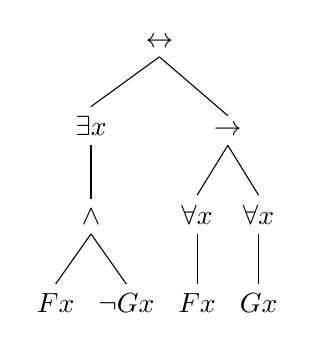
\begin{tikzpicture}
\tikzset{grow=down,level distance=32pt}
\Tree
[.\(\leftrightarrow\)
    [ .\(\exists x\)
        [ .\(\land\)
            [ .\(Fx\) ]
            [ .\(\neg Gx\) ]
        ]
    ]
    [.\(\rightarrow\)
        [.\(\forall x\)
            [.\(Fx\) ]
        ]
        [.\(\forall x\)
            [.\(Gx\) ]
        ]
    ]
]
\end{tikzpicture}
\end{figure}

The main logical operator is $\leftrightarrow$. 
The $\exists x$ in $\exists x (Fx \land \neg Gx)$ has scope over $Fx \land \neg Gx$

The $\forall x$ in $\forall x Fx$ has scope over $Fx$ and $\forall x Gx$ has scope over $Gx$.
The $\rightarrow$ in $\forall x Fx \rightarrow \forall xGx$ has scope over $\forall x Fx$ and $\forall xGx$.


\[ \forall x (Ax \leftrightarrow Bx) \rightarrow \exists (Ax \land Bx) \]

\begin{center}
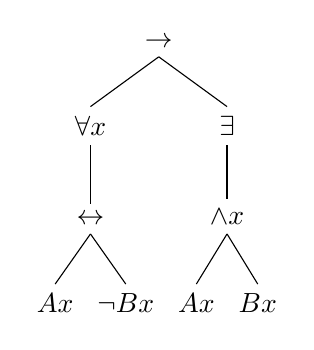
\begin{tikzpicture}
\tikzset{grow=down,level distance=32pt}
\Tree
[.\(\rightarrow\)
    [ .\(\forall x\)
        [ .\(\leftrightarrow\)
            [ .\(Ax\) ]
            [ .\(\neg Bx\) ]
        ]
    ]
    [.\(\exists\)
        [.\(\land x\)
            [.\(Ax\) ]
            [.\(Bx\) ]
        ]
    ]
]
\end{tikzpicture}
\end{center}


The main logical operator is $\rightarrow$. It's scope is over $\forall x (Ax \leftrightarrow Bx)$ and $\exists (Ax \land Bx)$.
The $\forall x$ in $\forall x (Ax \leftrightarrow Bx)$ has scope over $Ax \leftrightarrow Bx$.
The $\exists x$ in $\exists (Ax \land Bx)$ has scope over $Ax \land Bx$.
The $\leftrightarrow$ in $Ax \leftrightarrow Bx$ has scope over $Ax$ and $Bx$.
The $\land$ in $Ax \land Bx$ has scope over $Ax$ and $Bx$.


\[ (\forall x Fx \rightarrow \forall x Gx) \rightarrow \forall x (Fx \rightarrow Gx) \]

\begin{center}
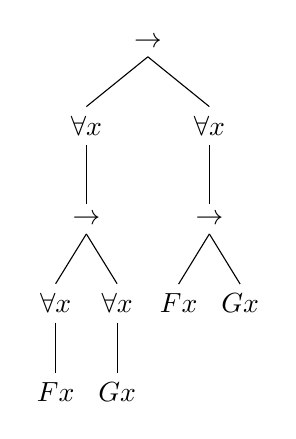
\begin{tikzpicture}
\tikzset{grow=down,level distance=32pt}
\Tree
[.\(\rightarrow\)
    [ .\(\forall x\)
        [ .\(\rightarrow\)
            [ .\(\forall x\)
                [ .\(Fx\) ]
            ]
            [ .\(\forall x\)
                [ .\(Gx\) ]
            ]
        ]
    ]
    [.\(\forall x\)
        [.\(\rightarrow\)
            [.\(Fx\) ]
            [.\(Gx\) ]
        ]
    ]
]
\end{tikzpicture}
\end{center}

The main logical operator is $\rightarrow$. It's scope is over $(\forall x Fx \rightarrow \forall x G)$ and $\forall x (Fx \rightarrow Gx)$.
The $\forall x$ in $\forall x Fx$ has scope over $Fx$.
The $\forall x$ in $\forall x Gx$ has scope over $Gx$.
The $\rightarrow$ in $\forall x Fx \rightarrow \forall x Gx$ has scope over $\forall x Fx$ and $\forall x Gx$.
The $\forall x$ in $\forall x (Fx \rightarrow Gx)$ has scope over $Fx \rightarrow Gx$.
The $\rightarrow$ in $Fx \rightarrow Gx$ has scope over $Fx$ and $Gx$.




\[ \forall x (Ax \rightarrow Bx) \lor \forall x( \neg Ax \rightarrow Bx) \]

\begin{center}
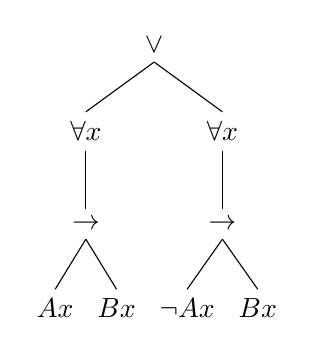
\begin{tikzpicture}
\tikzset{grow=down,level distance=32pt}
\Tree
[.\(\lor\)
    [ .\(\forall x\)
        [ .\(\rightarrow\)
            [ .\(Ax\) ]
            [ .\(Bx\) ]
        ]
    ]
    [.\(\forall x\)
        [.\(\rightarrow\)
            [.\(\lnot Ax\) ]
            [.\(Bx\) ]
        ]
    ]
]

\end{tikzpicture}
\end{center}

The main logical operator is $\lor$. It's scope is over $\forall x (Ax \rightarrow Bx)$ and $\forall x( \neg Ax \rightarrow Bx)$.
The $\forall x$ in $\forall x (Ax \rightarrow Bx)$ has scope over $Ax \rightarrow Bx$.
The $\forall x$ in $\forall x( \neg Ax \rightarrow Bx)$ has scope over $\neg Ax \rightarrow Bx$.
The $\rightarrow$ in $Ax \rightarrow Bx$ has scope over $Ax$ and $Bx$.
The $\rightarrow$ in $\neg Ax \rightarrow Bx$ has scope over $\neg Ax$ and $Bx$.
The $\neg$ in $\neg Ax$ has scope over $Ax$.


\section*{Solution to Problem 2}

Convert the following predicate logic sentences into English.

\[ \exists x (Fx \land \neg Gx) \]

There is a fish that doesn't have gills.

\[ \neg \exists x (Fx \land \neg Gx) \]

There is not a fish that doesn't have gills.

\[ \forall x Fx \rightarrow \forall x Gx \]

If everything is a fish, then everything has gills.

\[ \forall x (Fx \rightarrow Gx) \]

All fish have gills.

\[ \forall x ((Fx \land Tx) \rightarrow Gx) \]

Every fish with a tail has gills.

\[ \forall x ((Fx \lor Tx) \rightarrow Gx) \]

Every fish or tailed creature has gills.

\[ \forall x (Fx \lor \neq Fx) \]

Everything is either a fish or not a fish.

\[ \forall x Fx \lor \forall x \neg Fx \]

Either everything is a fish or nothing is a fish.


\section*{Solution to Problem 3}

Translate the following sentence from English into predicate logic. 

Some metals conduct electricity.
\[ \exists x (Mx \land Cx) \]

No metal conducts electricity.
\[ \neg \exists x (Mx \land Cx) \]

If some metal s don't conduct electricity, then it's not the case that all metals do conduct electricity

\[ (\exists x (Mx \land \neg Cx)) \rightarrow \neg (\forall x (Mx \land Cx)) \]

All hard metals conduct electricity.

\[ \forall x ((Hx \land Mx) \rightarrow Cx) \]

All metals and plastics conduct electricity.

\[ \forall x ((Mx \lor Px) \rightarrow Cx) \]

Rhinos exist, but unicorns do not.

\[ \exists x Rx \land \neg \exists x Ux \]

\section*{Solution to Problem 5}

State the truth-values of the listed

sentences on the following interpretation:

Domain = {1, 2, 3, 4, 5}


$F \rightarrow \{1, 2\}$

$G \rightarrow \{1, 2, 3, 4\}$

$L \rightarrow \{<1,1>, <1,2>, <1,3>, <1, 5>, <2, 2>, <3, 1>, <3,2>,<4, 2>, <5, 2>\}$

$a \rightarrow 2$

\[ \forall x Gx \]
False, 5 is not in G.

\[ \forall x(Fx \rightarrow Gx) \]
True, all elements of F are in G.

\[ \exists x(Gx \land \lnot Fx) \]
True, Every element is either in G or not in F.

\[ \forall x F x \rightarrow \forall x G x \]
True, the condition is false. 

\[ \forall x Lxa \]
True, L maps every value in x to the value 2

\[ \forall x Lax \]
False, L doesn't map 2 to every value in x

\[ \forall x Lxx \]
False, L doesn't map 3 to itself

\[ \forall x(Fa \rightarrow Lax) \]
False, L doesn't map 2 to every value in x


\section*{Solution to Problem 6}

Use the tree test to verify that each of the following argumens is valid. 

\[ \forall x (Fx \rightarrow Gx), \neg Ga, \therefore \neg Fa \]





\section*{Solution to Problem 7}

Prove rule-soundness of the tree rules for the conditional and the negated conditional.

Rule Soundness: if the premise/input is true in some case/valuation C, then all the lines in at least
one of its conclusions/outputs is true in case C too.




\section*{Solution to Problem 8}
 Prove the rule-completeness of the tree rules for the biconditional and the negated biconditional.  
 
Rule Completeness:  If all the lines in one of its conclusions/outputs  is true in some case/valuation 
C, the premise/input is true in C also.



\section*{Solution to Problem 9}



\end{document}

